\chapter{Experiment and Result}
\section{Experiment}
\subsection{Tools Used}
To process the EEG signal, there are a wide variety of devices that can be used in EEG data processing, among others:

\subsubsection{EEG amplifier Mitsar -202 and WinEEG}
For the EEG signal acquisition phase in this study, the hardware used is an EEG amplifier Mitsar-202 32 channels. Display devices of this amplifier can be observed in Figure 5.1
\begin{figure}[h!]
\centering
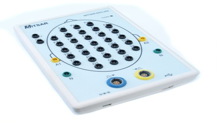
\includegraphics[scale=0.5]{figures/51.PNG}
\caption{EEG amplifier system Mitsar-202}
\label{labelgambar5}
\end{figure}

\par
To record EEG signals using this amplifier, the amplifier device is connected to a PC using USB. Furthermore, speakers WinEEG operated via software on the PC. WinEEG program display can be observed in Figure 5.2.
\begin{figure}[h!]
\centering
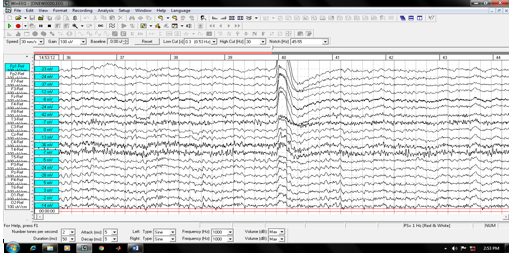
\includegraphics[scale=0.5]{figures/52.PNG}
\caption{Display software WinEEG}
\label{labelgambar6}
\end{figure}

\subsubsection{ Electro-Cap}
\par
Electro-Cap a hat-shaped device that serves to facilitate the placement of EEG electrodes. This device consists of some lead electrodes connected to an amplifier via adapters (Electro-Cap International, Inc., 2015). Views Electro-Cap can be observed in Figure 5.3
\begin{figure}[h!]
\centering
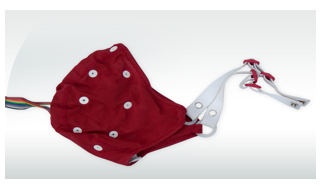
\includegraphics[scale=0.5]{figures/53.PNG}
\caption{Electro-Cap}
\label{labelgambar7}
\end{figure}

\subsubsection{MATLAB}
\par
MATLAB is a high-level programming language for applications in various fields, such as numeric computation, analysis, and data visualization software and algorithm development, and design of the model system. (MathWorks, 2017) MATLAB toolbox is complemented by a wide range to support specific tasks, either developed directly by MathWorks and third parties. In this study, the toolkit is used field trip.

\par
The field trip is an open source software for EEG analysis, magnetoencephalography (MEG), electrophysiological data and more. The software supports a variety of functions for the study of EEG as a pre-processing of data, ERP analysis, classification, and others. Here is a preview of the software is MATLAB icon 2017.
\begin{figure}[h!]
\centering

\includegraphics[scale=0.6]{figures/54.PNG}
\caption{The initial view Matlab}
\label{labelgambar8}
\end{figure}

\section{Data Processing}
\subsection{Pre-Processing}
\par
Pre-processing is beginning the process of signal processing that consists of raw, and bandpass filter and Brain Mapping. Such procedures would improve the signal by removing artifacts, and present signals are more easily analyzed.

\subsubsection{raw Data}
\par
To record EEG signals using this amplifier, the amplifier device is connected to a PC using USB. Furthermore, speakers WinEEG operated via software on the PC. WinEEG program display can be observed in Figure 5.5
\begin{figure}[h!]
\centering
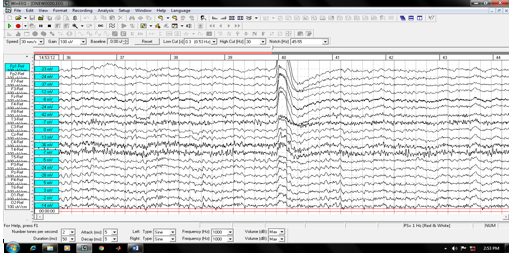
\includegraphics[scale=0.6]{figures/52.PNG}
\caption{Example of Display Raw Data Subject}
\label{labelgambar9}
\end{figure}

\par
Raw Data is the raw data that has not been treated at all. Wave signal is still very rough and irregular caused by artifacts in the message. Raw EEG signal data on each channel can be seen
\begin{figure}[h!]
\centering
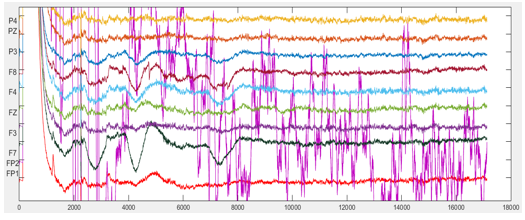
\includegraphics[scale=0.6]{figures/55.PNG}
\caption{Example of Display Raw Data Subject}
\label{labelgambar10}
\end{figure}

\subsubsection{bandpass Filter}
\par
Bandpass filter with a frequency range of 3 Hz to 30 Hz is used to the raw data. Bandpass filters on the EEG signals are shown in Figure 5.6
\begin{figure}[h!]
\centering
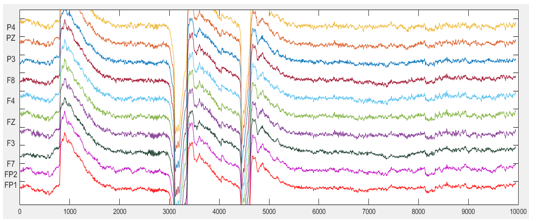
\includegraphics[scale=0.6]{figures/56.PNG}
\caption{Display EEG data after Bandpass Filter}
\label{labelgambar10}
\end{figure}

\subsection{Data Processing Using Wavelet}
\par
The wavelet transform is a method of signal processing requires the workings resemble signal analysis using the Fourier transform by splitting the signal to be analyzed into several parts. The difference, tell the Fourier transform of a signal frequency information, but not with the timing information but the wavelet transform signal in the time domain into signals in the time and frequency, in this case, is formed into an area of translation and scale. Translation (reading) is a form of transformation from the time domain translation associated with the location of the window function, where window be moved along the incoming signal. Scale (scale) is a form of transformation of frequency, where the value scales inversely proportional to the frequency value.

\section{Result}
\par
At this stage, to see the most dominant brain activity. Here is a scene Wavelet application configuration and the results of Brain Mapping one subject

\begin{enumerate}
 \item Result Rilex Close Pre
     \begin{figure}[h!]
\centering
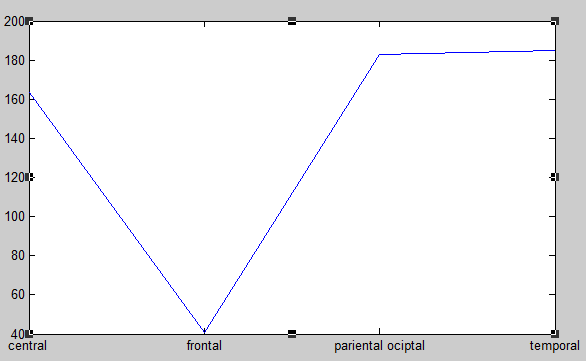
\includegraphics[scale=0.6]{figures/hasil1.PNG}
\caption{The Brain Sigbal Rilex Close Pre}
\label{labelgambar5}
\end{figure}

\par
picture Result Rilex Close Pre above is the result of processing data using wavelets. the graph above is the result of recording subject 1 data in relaxed and closed eyes. in this condition, the subject is told to close his eyes and not think of anything. after recording and processing data, the subject's brain condition can be seen based on the picture above. the result, the central subject brain condition is 160Hz, Frontal 40Hz and the ociptal Pariental is at 180Hz

\item Result Rilex Close Post after 4 minutes
\begin{figure}[h!]
\centering
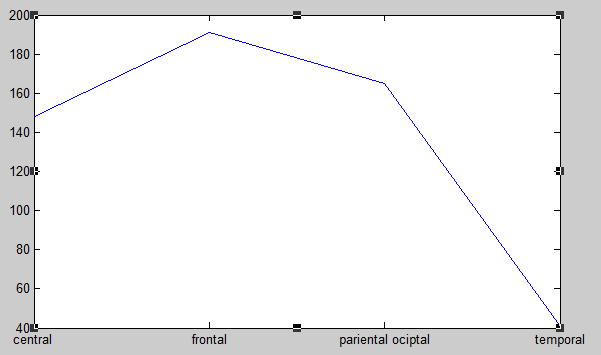
\includegraphics[scale=0.6]{figures/hasil2.PNG}
\caption{The brain signals Rilex Close Post after 4 minutes}
\label{labelgambar12}
\end{figure}

\par
picture Result Rilex Close Post after 4 minutes above is the result of processing data using wavelets. The graph above is the result of recording subject 1 data after the administration of methadone for 4 minutes. in this condition, data in colleagues used WinEEG on subjects who had been given methadone. after recording and processing data, the subject's brain condition can be seen based on the picture above. As a result, the central subject brain condition is 150Hz, Frontal 190Hz, Ociptal Pariental is at 160Hz and temporally 40Hz
\item Result Rilex close post after 65 minutes
\begin{figure}[h!]
\centering
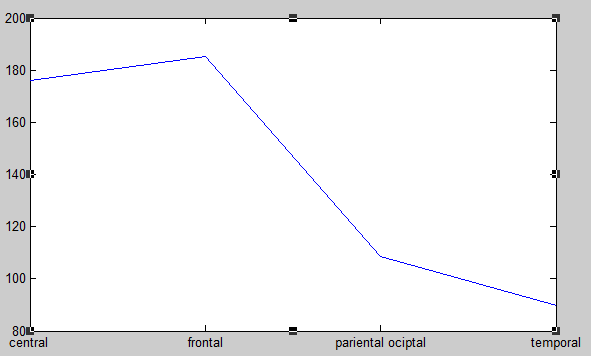
\includegraphics[scale=0.6]{figures/hasil3.PNG}
\caption{Rilex Close Post after 65 minutes}
\label{labelgambar13}
\end{figure}

\par
picture Result Rilex close post after 65 minutes above is the result of processing data using wavelets. the graph above is the result of recording subject 1 data after giving methadone for 65 minutes. in this condition, data in colleagues used WinEEG on subjects who had been given methadone. after recording and processing data, the subject's brain condition can be seen based on the picture above. As a result, the central subject brain condition is 160Hz, Frontal 200Hz, and the ociptal Pariental is at 110Hz.
   
\end{enumerate}

    